%!TEX root = main.tex

\chapter{Estado del arte}
\section{Particle Swarm Optimization}
Como se introduce en el artículo de Kaveh \cite{Psoexplain14}, el algoritmo \emph{Particle Swarm Optimization} es una meta-heurística inspirada en las observaciones de la naturaleza acerca del comportamiento social de poblaciones de enjambres. Esta abstracción está basada en la interacción en grupo de seres vivos, por ejemplo, las gaviotas, las cuales suelen moverse en bandadas, vuelan en conjunto cerca del mar en búsqueda de zonas donde hayan alimento (peces), moviéndose individualmente, pero siendo influenciadas o guiadas por otras. El método simula la conducta de los individuos a través de partículas que se mueven dentro de un espacio (rango de posibles valores conocido como espacio de búsqueda), siendo estas afectadas por factores individuales (conocimiento propio del lugar donde estoy) y factores colectivos (conocimiento del enjambre del mejor lugar encontrado), los cuales dirigen el movimiento de estos grupos a zonas las cuales son escogidas o determinadas por una función objetivo (\emph{fitness function}).\\
Para cada partícula su vector posición  $\vec{x}$ representa una solución candidata, la cual varía dentro del espacio de búsqueda a velocidad $\vec{v}$. Después de varias iteraciones, el enjambre o conjunto de partículas se irá concentrando en aquellas zonas donde las posiciones obtengan mejores puntajes al ser evaluadas por la función objetivo.
\\El modelo clásico presentado por Kennedy y Eberhart\cite{Kennedy95}, describe la variación de la velocidad y de la posición de las partículas como se presenta a continuación:
\begin{align}
    v_{i,j}^{k+1} &= v_{i,j}^{k} + c_{1}r_{1}(xbest_{i,j}^k - x_{i,j}^k) + c_{2}r_{2}(xgbest_{j}^{k} - x_{i,j}^k) \\
    x_{i,j}^{k+1} &= x_{i,j}^{k} + v_{i,j}^{k+1}
\end{align}    
Como se explica en Kaveh \cite{Psoexplain14} $x_{i,j}^{k}$ y $v_{i,j}^{k}$ son la $j$-ésima componente de la posición y la velocidad de la partícula $i$ respectivamente en la iteración o tiempo $k$, $r_{1}$ y $r_{2}$ son número aleatorios uniformes que varían de 0 a 1, $xbest_i$ y $xgbest$ representan las mejores soluciones alcanzadas por la partícula $i$ y por el enjambre en conjunto respectivamente, $c_1$ y $c_2$ son parámetros que representan la confianza en la solución individual de la partícula (parámetro cognitivo) y la incidencia del aspecto colectivo o solución global (parámetro social), respectivamente. Un esquema de la interacción de estos componentes se aprecia en la figura \ref{fig:move_part}\\
\begin{figure}[h!]
    \centering    
    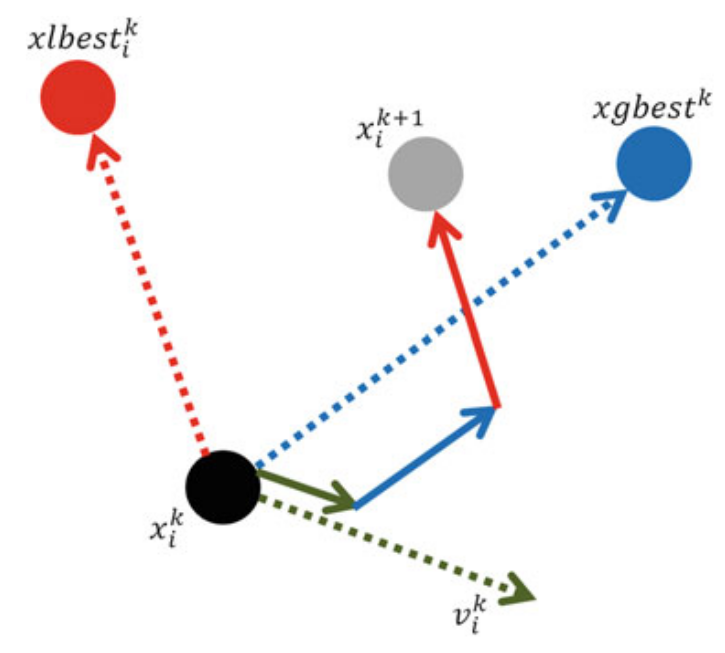
\includegraphics[height=50mm]{figures/move_particle.png} 
    \caption{Movimiento de una partícula}
    \vspace{-.25cm} 
    \caption*{Creado por Kaveh\cite{Psoexplain14}.}
    \label{fig:move_part}
\end{figure}
El modelo clásico presentado tiene ciertas deficiencias, en particular la forma en que se actualiza la velocidad no considera una ponderación para el aporte de la velocidad previa en una partícula. Para corregir esto, simplemente se añade un factor que escala la velocidad previa. Como se explica en Kaveh \cite{Psoexplain14}, este peso que se añade a la velocidad previa permite tener un control más apropiado respecto al comportamiento del enjambre. En términos extremos, si la velocidad previa se elimina (peso nulo), las partículas quedan atrapadas en una región local, pero si se le da demasiado peso, converge rápidamente a un óptimo local.\\
Es por esto que la forma del PSO actual tiene un parámetro $w$ que representa la incidencia de la velocidad previa en la velocidad actual de la partícula (parámetro llamado factor de inercia). Nuevamente, se tiene que la partícula actualiza su velocidad de la siguiente forma: 
\begin{align}\label{eq:PSO}
    v_{i,j}^{k+1} &= wv_{i,j}^{k} + c_{1}r_{1}(xbest_{i,j}^k - x_{i,j}^k) + c_{2}r_{2}(xgbest_{j}^{k} - x_{i,j}^k)\\
    x_{i,j}^{k+1} &= x_{i,j}^{k} + v_{i,j}^{k+1}
\end{align}    
Donde $w$ es el factor conocido como ``inercia'' de la partícula, y regula la incidencia de la velocidad previa en la actual, tal como podría esperarse de una partícula en aceleración.\\
A modo de complemento, en el trabajo inicialmente citado, se puede observar una revisión completa del estado del arte del método \emph{Particle Swarm Optimization} en términos de diseño o arquitectura del algoritmo, donde se exponen las distintas modificaciones y alternativas existentes en la literatura que pretenden mejorar aspectos como:
\begin{enumerate}
    \item  Configuración de parámetros (inercia, cognitivo, social, aleatorios).
    \item  Problemas asociados a la convergencia prematura.
    \item  Estructura de algoritmo o topologías que modifican la comunicación entre partículas (o la incidencia de las soluciones globales y particulares).
    \item  Sesgos en la búsqueda por la forma de la región o por la interacción de las partículas (operadores de combinación como el promedio, que tienden a centrar la búsqueda en determinada región).
    \item  Algoritmos híbridos con PSO.
    \item  Versión discreta del PSO. 
\end{enumerate}  

\section{Velocidad del viento}
\subsection{Distribución de Weibull}
Dado un conjunto de datos de velocidad obtenidos de la medición del viento, se puede crear un histograma que represente la frecuencia de estos datos. A partir de esto, es posible ajustar un modelo probabilístico (distribución de densidad de probabilidad) que explique el comportamiento de las velocidades del viento medido. Dicho modelo comúnmente se basa en la distribución de Weibull, la cual es ampliamente aceptada por la comunidad dedicada al estudio meteorológico, tal y como se menciona en el trabajo de Carneiro et al. \cite{Carneiro15}, Kongnam et al. \cite{Kongnam15}, Dabbaghiyan et al.\cite{Dabbaghiyan15}, Fadare \cite{Fadare08}, Weisser \cite{Weisser02} y Chang \cite{Chang10_2}. En el trabajo realizado por Carneiro et al. \cite{Carneiro15}, se describe la distribución de Weibull como: 
 \begin{align}\label{eq:weibull}
     f_{weibull}(v) = \frac{k}{c} \cdot (\frac{v}{c})^{k-1} \cdot e^{-(\frac{v}{c})^ k}
 \end{align}
 Donde $k$ y $c$ son los parámetros de ajuste que representan la forma y la escala (o amplitud) de la distribución respectivamente, y $v$ es el valor de la velocidad del viento a la que el modelo asociará una determinada densidad. Un ejemplo de como varia la forma de esta distribución se aprecia en la figura \ref{fig:weibull_fig}, en donde se ven distintas curvas de Weibull, con diferentes parámetros $k$ manteniendo $c$ constante.
\begin{figure}[h!]
    \centering    
    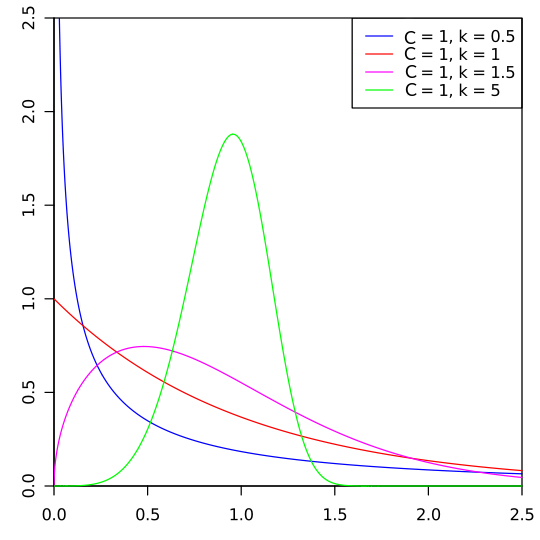
\includegraphics[height=50mm]{figures/weibull_distribution.png} 
    \caption{Función de distribución de probabilidad de Weibull}
    \vspace{-.25cm} 
    \caption*{Adaptación propia desde \cite{wikiWeibull}.}
    \label{fig:weibull_fig}
\end{figure}
 \subsection{Métodos numéricos}  \label{subsec:Numeric_Methods}
 Tradicionalmente, se utilizan métodos numéricos para estimar los parámetros de la distribución de Weibull. En el artículo de Chang \cite{Chang10}, se realiza una comparación de seis métodos numéricos comúnmente utilizados para la obtención de $k$ y $c$. A continuación, se describen brevemente estos métodos:
 \begin{enumerate}
     \item \textbf{The Moment}: Se basa en la iteración numérica de las siguientes dos ecuaciones:
        \begin{align}
            \bar{v} &= c\Gamma(1 + \frac{1}{k})\\
            \sigma &= c[\Gamma(1 + \frac{2}{k}) - \Gamma^2(1 + \frac{1}{k})]^{\frac{1}{2}}
        \end{align}    
        Donde $\bar{v}$ es el promedio y $\sigma$ la desviación estándar de los datos de velocidad del viento.
    \item \textbf{Empirical}: Considerado un caso especial del método del momento. Los parámetros son calculados de la siguiente forma: 
        \begin{align}
            k &= (\frac{\sigma}{\bar{v}})^{-1.086}\\
            c &= \frac{\bar{v}}{\Gamma(1 + \frac{1}{k})}
        \end{align}    
    \item \textbf{Graphical}: Se ajustan rectas a los datos de velocidad del viento usando mínimos cuadrados. Con una doble transformación logarítmica, la función de distribución acumulativa queda:
        \begin{align}
            \ln\{-\ln[1- F(v)]\} = k\ln(v) - k\ln(c)
        \end{align}    
         Realizando un gráfico para $ln(v)$ en vez de $ln(-ln(1-F(v)))$, la pendiente de la recta que se ajusta mejor a los pares de datos es el parámetro de la forma de la distribución de Weibull. El parámetro de escala se obtiene por la intersección con la coordenada $y$.  
    \item \textbf{Maximum likelihood}: En este método, son necesarias muchas iteraciones. Los parámetros de Weibull están dado por:
        \begin{align}
            k &= [\frac{\sum_{i=1}^n v_i^k \ln(v_i)}{\sum_{i=1}^n v_i^k} - \frac{\sum_{i=1}^n \ln(v_i)}{n}]^{(-1)}\\
            c &= (\frac{1}{n}\sum_{i=1}^n v_i^k)^{\frac{1}{k}}
        \end{align}    
         Donde $v_i$ es la velocidad del viento en el paso $i$ y $n$ es el número de puntos de datos distintos de cero. 
    \item \textbf{Modified maximum likelihood}: Este método es utilizado si es que se tiene disponible los datos de velocidad del viento en una distribución de frecuencias. Los parámetros de Weibull son calculados como:
        \begin{align}
            k &= [\frac{\sum_{i=1}^n v_i^k \ln(v_i)f(v_i)}{\sum_{i=1}^n v_i^kf(v_I)} - \frac{\sum_{i=1}^n\ln(v_i)f(v_i)}{f(v \geq 0)}]^{-1}\\
            c &= [\frac{1}{f(v \geq 0)}\sum_{i=1}^n v_i^{k}f(v_i)]^{1/k}
        \end{align}
         Donde $v_i$ es la velocidad del viento central al intervalo $i$, $n$ es el número de intervalos. $f(v_i)$ es la frecuencia de la velocidad del viento dentro del intervalo $i$ y $f(v \geq 0)$ la probabilidad de que la velocidad del viento sea mayor o igual a cero.
    \item \textbf{Energy pattern factor method}: El factor del patrón de energía es definido como:
        \begin{align}
            E_{pf} = \frac{\bar{v^3}}{\bar{v}^3}
        \end{align}   
         Donde $\bar{v^3}$ es el promedio de las velocidades del viento cúbicas. Los parámetros de Weibull pueden ser calculados como:
        \begin{align}
            k &= 1 + \frac{3.69}{E_{pf}^2}\\
            c &= \frac{\bar{v}}{\Gamma(1 + \frac{1}{k})}
        \end{align}    
 \end{enumerate}     
 Estos métodos fueron comparados a través de pruebas de desempeño, usando una simulación basada en el método de Montecarlo. El análisis de los datos del viento fue desarrollado bajo criterios tales como el test Kolmogorov-Smirnov, \emph{parameter error}, \emph{root mean square error} y el error de energía del viento. De ello, bajo distintas condiciones, ciertos métodos se comportan mejor que otros al momento de ajustar la distribución de Weibull a los datos de prueba. \\
 En la búsqueda de nuevas alternativas surge una propuesta para mejorar el ajuste de la función de distribución de probabilidad a los datos, a través del uso de la meta-heurística \emph{Particle Swarm Optimization}, propuesta que mejora la calidad de los resultados en comparación con los métodos numéricos presentados.  
 \subsection{Particle Swarm Optimization}
 En Carneiro et al. \cite{Carneiro15}, se realiza un caso de estudio de las características del viento en las zonas costeras de Parnaiba y Maracanaú, y en una zona interior, Petrolina, en Brasil. Allí se explica la necesidad de obtener un modelo para el comportamiento estocástico del viento, de manera de poder evaluar el potencial energético de aquellas regiones. Tal y como se adelanta anteriormente, el modelo utilizado para este propósito es la distribución de Weibull. Para poder utilizar dicha distribución, es necesario ajustar los parámetros del modelo a los datos recolectados.\\
 En el estudio mencionado, se propone un \emph{particle swarm optimization} para encontrar los parámetros $k$ y $c$ de la distribución de Weibull y a su vez corroborar que la calidad de la solución encontrada por el PSO, comparada con los métodos numéricos tradicionales, es de mejor calidad.\\
 Así, se define la función de aptitud para el PSO como:
\begin{align}\label{eq:PSO_FO}
    \epsilon(v_i) = \frac{1}{2}\sum_{i=0}^{n}(f_{real}(v_i) - f_{weibull}(v_i))^2
\end{align}
Donde $\epsilon$, es el error cuadrático a minimizar entre los valores del histograma de los datos recolectados y la función de distribución de Weibull.\\
El PSO utilizado es el modelo clásico presentado en la sección anterior, considerando los parámetros $w, c1$ y $c2$, sin embargo, para controlar la convergencia del método, se establece que estos parámetros varíen durante la ejecución del algoritmo dentro de un rango definido ($w \in \{0.4, 0.9\}, c1$ y $c2 \in \{0, 2.5\}$), aumentando los factores de inercia y cognitivo, y disminuyendo el factor social a medida que se avanza en las iteraciones. Esto se traduce en que se explotan las soluciones iniciales, para posteriormente en iteraciones finales el algoritmo explore en una vecindad local al óptimo encontrado hasta el momento.\\
Finalmente, para evaluar los resultados de la propuesta, se compara el PSO con cinco de los seis métodos numéricos mencionados en la sección \ref{subsec:Numeric_Methods} utilizados para la estimación de los parámetros de Weibull: \emph{Moment Method} (M), \emph{Energy Method} (E), \emph{Energy Pattern Factor Method} (EPF), \emph{Energy Equivalent Method} (EE) y \emph{Maximum Likelihood} (ML). Además, para medir la calidad de cada método, se utilizan tres \emph{test} estadísticos: \emph{correlation} (r), \emph{relative bias} (RB) y \emph{root mean square error} (RMSE).\\
Los resultados que se exponen en el trabajo citado demuestran que mediante la meta-heurística \emph{particle swarm optimization} se pueden obtener los mejores parámetros de ajuste para la distribución de Weibull. Un ejemplo de esto es expuesto en la figura \ref{fig:pso_fit}.
\begin{figure}[h!]
    \centering    
    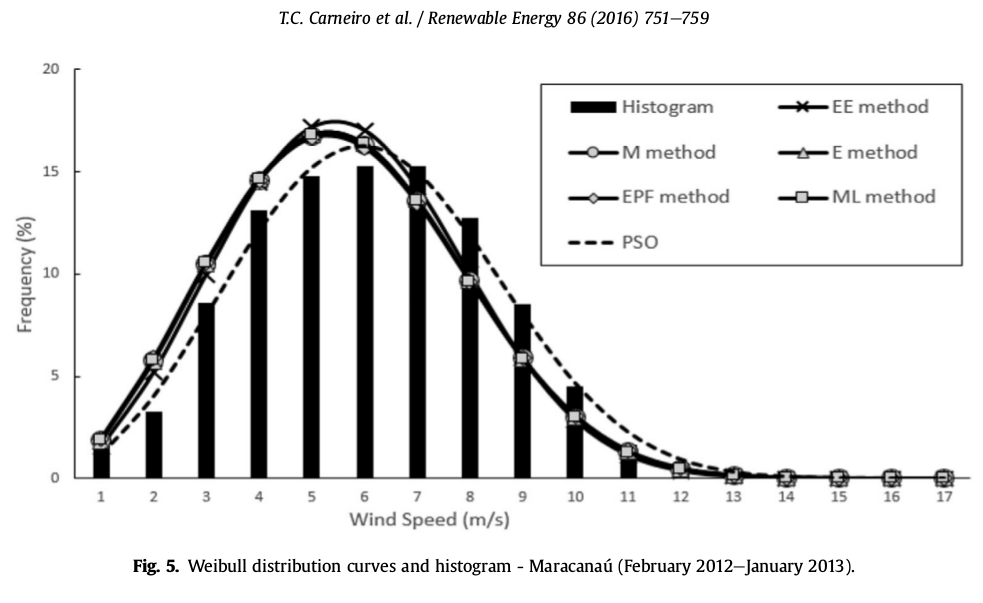
\includegraphics[height=50mm]{figures/pso_fit.png} 
    \caption{Distribución de Weibull con histograma - Maracanaú}
    \vspace{-.25cm} 
    \caption*{Creado por Carneiro et al.\cite{Carneiro15}.}
    \label{fig:pso_fit}
\end{figure}
En Kongnam et al. \cite{Kongnam15}, el PSO es utilizado para el problema del control de la velocidad de las turbinas de viento para maximizar la generación de energía. En este trabajo, se utiliza la distribución de Weibull para el modelado de la velocidad del viento. La construcción del PSO es llevada a cabo considerando el problema de la convergencia prematura, por lo que se desarrollan funciones que varían estos parámetros a lo largo de la ejecución.\\

\section{Dirección del viento}
En el trabajo acerca del modelado del comportamiento de la dirección del viento en Malasia \cite{Winddirelse15}, se propone que para identificar la(s) dirección(es) dominante del viento se utilice la función de densidad de probabilidad \emph{finite von Mises-Fisher} (FVMF) ajustada a las mediciones obtenidas. Estos datos acerca del viento fueron obtenidos desde cinco estaciones meteorológicas ubicadas en distintas zonas en la península de Malasia.\\
La FVMF, o la función de densidad de probabilidad de von Mises como también se le llamará más adelante, de forma genérica, está definida de la siguiente forma:
\begin{align}
    f(x;\mu_{h}, k_{h}) = \sum_{h=1}^{H}(w_{h})\frac{k^{\frac{d}{2} - 1}}{(2\pi)^{\frac{d}{2}}I_{\frac{d}{2} - 1} (k)}e^{(k_h\mu_{h}^{T}x)}
\end{align}    
Donde $x=[cos(\theta_i), sin(\theta_i)]$, $\frac{k^{\frac{d}{2} - 1}}{(2\pi)^{\frac{d}{2}}I_{\frac{d}{2} - 1} (k)}$ es una constante de normalización, $d$ es la dimensión del vector aleatorio $x$ ($d = 2$, para este caso), $\mu_{h}$ es el parámetro de dirección predominante (análogo a la media $\mu$ en la distribución normal), $k_h$ es el parámetro de concentración (análogo al recíproco de la dispersión $\sigma^{2}$), estos dos últimos para cada $h = 1, 2,...,H$ componente del FVFM y $w_h$ es el parámetro de mezcla o peso de las funciones de von Mises (\emph{mixture parameter}).\\
Además, el parámetro de mezcla del FVMF está sujeto a la siguiente restricción:
\begin{align}\label{eq:WeightConstraint}
    0 \leq w_h \leq 1 \text{ y } \sum_{h=1}^{H} w_{h} = 1 \text{ para } (h=1,2,...,H) 
\end{align}
Para estimar los parámetros del FVMF, se sugiere utilizar el método \emph{expectation maximization}, debido a que los métodos regulares son incapaces de manejar la complejidad del modelo, consideraciones que se mencionan en el trabajo de Banerjee et al.\cite{Banerjee05}.\\
Por último, los resultados de este trabajo muestran que FVMF provee un razonable ajuste a diferentes conjunto de datos, obteniendo un modelo que explica más del $90\%$ de la variación de los datos, en este caso, obtenidos de estaciones ubicadas en la península de Malasia. En la figura \ref{fig:wind_dir_vonMises} se aprecia el ajuste del modelo a los datos, tanto la comparación con el histograma, como en su versión circular.\\
\begin{figure}[h!]
    \centering    
    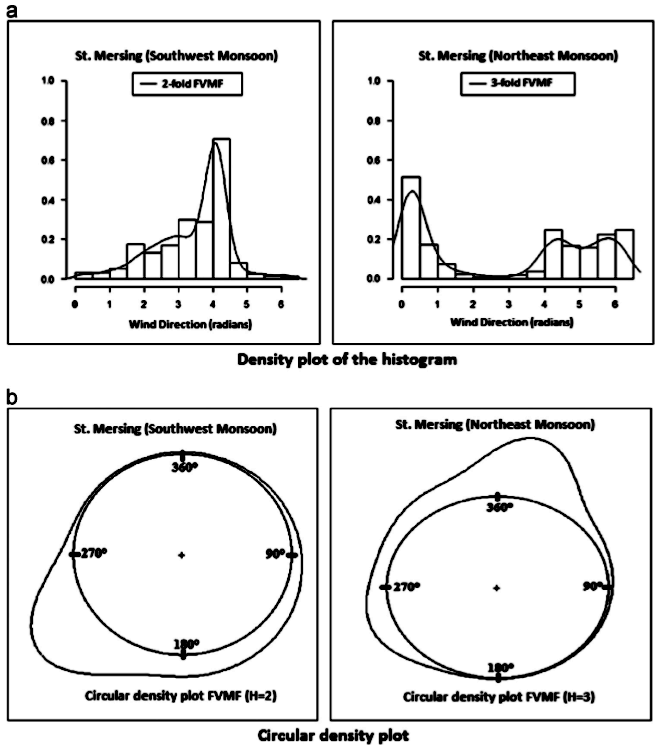
\includegraphics[height=100mm]{figures/wind_dir_vonMises.png} 
    \caption{Modelo de ajuste FVMV para suroeste y noreste en la estación Mersing}
    \vspace{-.25cm} 
    \caption*{Creado por \cite{Winddirelse15}.}
    \label{fig:wind_dir_vonMises}
\end{figure}

En el trabajo de Heckenbergerova et al.\cite{Heckenbergerova15}, se utiliza una estrategia diferente a la anteriormente mencionada, basados en la ya mencionada meta-heurística inspirada en la biología, \emph{Particle Swarm Optimization}. Proponen una forma distinta para encontrar un modelo de ajuste, utilizando la distribución estadística \emph{finite mixture of circular normal von Mises} (MvM), o simplemente \emph{mixture of von Mises distribution}, similar a la mencionada previamente.\\ 
En este caso, se define la \emph{simple von Mises distribution} (SvM) como:
\begin{align}\label{eq:simpleVonMises}
    f(\theta; \mu, k) = \frac{1}{2{\pi}I_{0}(k)}e^{k cos(\theta - \mu)}
\end{align}    
Donde $k \geq 0$, $0 \leq \mu \leq 2\pi$, $0 \leq \theta \leq 2\pi$ y $I_0(k)$ representa la versión modificada de la función de Bessel de primera clase y orden cero:
\begin{align}
    I_0(k) = \frac{1}{\sqrt{2\pi}}\int_0^{2\pi} e^{k cos(\theta)} d\theta = \sum_{k=0}^{\infty} \frac{1}{(k!)^2}(\frac{k}{2})^{2k}
\end{align}    
Para $k=0$, la distribución SvM se vuelve uniforme alrededor de un círculo con todas las direcciones equi-probables. Cuando una colección de datos tiene más de una dirección predominante, es necesario utilizar una mezcla (\emph{mixture}) de distribuciones.
Así, la función de densidad de probabilidad \emph{finite mixture of simple von Mises} (MvM-pdf) queda como:
\begin{align}\label{eq:mixtureVonMises}
    \phi(\theta; v) = \sum_{j=1}^{k} w_j \cdot f_j(\theta; \mu_j, k_j)
\end{align}    
Donde $k$ es el número de funciones de la mezcla, $j$ es el índice de una particular SvM-pdf con parámetros $\mu_j$ y $k_j$, $\theta$ es una variable angular ($0 \leq \theta \leq 2\pi$), y $v$ es un vector parámetro de la forma:
 \begin{align}\label{eq:sol_pso}
    v = (\mu, k, w) = (\mu_1, ..., \mu_k,k_1,...,k_k,w_1,...,w_k)
\end{align}
Para lograr el objetivo, se obtiene en primer lugar una aproximación numérica de los parámetros del MvM a partir de los datos recolectados de la dirección del viento, estrategia nombrada como estimación analítica en el trabajo de Heckenbergerova et al. \cite{Heckenbergerova15}. Luego optimiza estos parámetros mediante el uso de la meta-heurística \emph{particle swarm optimization}, con parámetros fijos, en donde la solución está representada por una codificación del vector $\vec{v}$ mencionado anteriormente\ref{eq:sol_pso}.\\ 
Como test estadístico, es utilizado el \emph{Pearson's chi-squared goodness-off-fit}. Los resultados muestran la mejora que se logra a la estimación inicial, comparando estos resultados con otra propuesta similar la cual se expone en un trabajo previo de los mismos autores \cite{Heckenbergerova13}, en donde se utiliza la misma estrategia pero reemplazando el PSO con algoritmos genéticos. Sin embargo, estos resultados no consiguen pasar el test estadístico impuesto por ellos mismos, por lo que existe trabajo futuro  a realizar para mejorar la propuesta y lograr la precisión deseada.\\
Los resultados obtenidos para los datos recolectados en el aeropuerto de St John localizado en Newfoundland, Canadá, son apreciables en la figura \ref{fig:dir_pso}.
\begin{figure}[h!]
    \centering    
    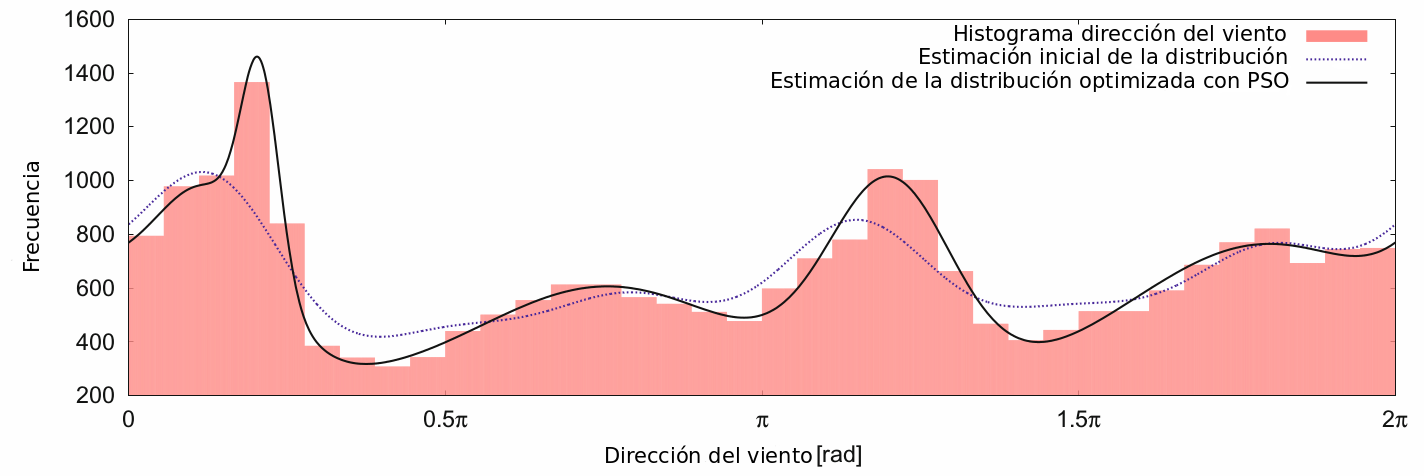
\includegraphics[height=50mm]{figures/dir_pso.png} 
    \caption{Ajuste dirección del viento, aeropuerto St. John}
    \vspace{-.25cm} 
    \caption*{Creado por Heckenbergerova et al.\cite{Heckenbergerova15}.}
    \label{fig:dir_pso}
\end{figure}

%%TODO explicar trabajo de los españoles...
Otro trabajo interesante de revisar es el caso de estudio realizado por Carta et al. \cite{Carta07}, en donde se utiliza la \emph{finite mixture of von Mises distribution} para representar la velocidad direccional de viento. El ajuste es realizado mediante el método de mínimos cuadrados, y resuelto con el algoritmo Levenberg-Marquardt \cite{Gavin16} el cual requiere de un punto de partida o solución inicial. Para ello, utilizan el mismo método que se propone en el trabajo de \cite{Heckenbergerova13} el cual se utiliza en este trabajo y que es explicado en la siguiente sección \ref{ss:model_math_dir}. La calidad de la solución es medida a través del test $R^2$, y dentro de las conclusiones que se obtienen, es que más de 6 mezclas\emph{mixtures} de von Mises no incrementan considerablemente el valor de $R^2$\\
El método es aplicado a datos recolectados desde dos estaciones del clima en el archipiélago de las islas Canarias. Una vez más, se confirma que la \emph{finite mixture of von Mises distribution} es aplicable a distintas regiones con una o más direcciones predominantes. 